Earth observing satellites play an important role for many scientific and
meteorological applications. Their unique capability to provide frequent
observations of large parts of the globe allows meteorologists to predict the
weather and scientists to study the Earth and its atmosphere. Weather
predictions as well as the monitoring of the Earth's climate are of considerable
societal and economical value; a value that is likely to increase as the Earth's
climate warms.

The observations made by Earth-observing satellites consist of measurements of
electromagnetic radiation, which is either reflected or emitted from the Earth
and its atmosphere. An example of such measurements is given in
Fig.~\ref{fig:introduction:water_vapor}. Besides demonstrating the delicate
beauty of the Earth and its atmosphere, this image can inform a trained eye
about their physical state. The image shows infrared radiation emitted from a
low pressure system over the Mediterranean sea. The measured signal in this
example is the intensity of the radiation, represented from intense to weak by
the bright to dark coloring. At this specific wavelength, the measured radiation
stems from water vapor and clouds in the atmosphere. Dry air, which contains
less water vapor, appears less opaque at this frequency. The more intense
radiation thus stems from lower down in the atmosphere where temperatures are
higher thus marking regions of relatively dry air. Moist air, which is more
opaque, emits radiation from higher up in the atmosphere where temperatures are
lower and thus produces the moderate intensities in the image. The lowest
intensities stem from high clouds which, due to their opacity, emit radiation at
very high altitudes and cold atmospheric temperatures.

\begin{figure}[h!]
\centering
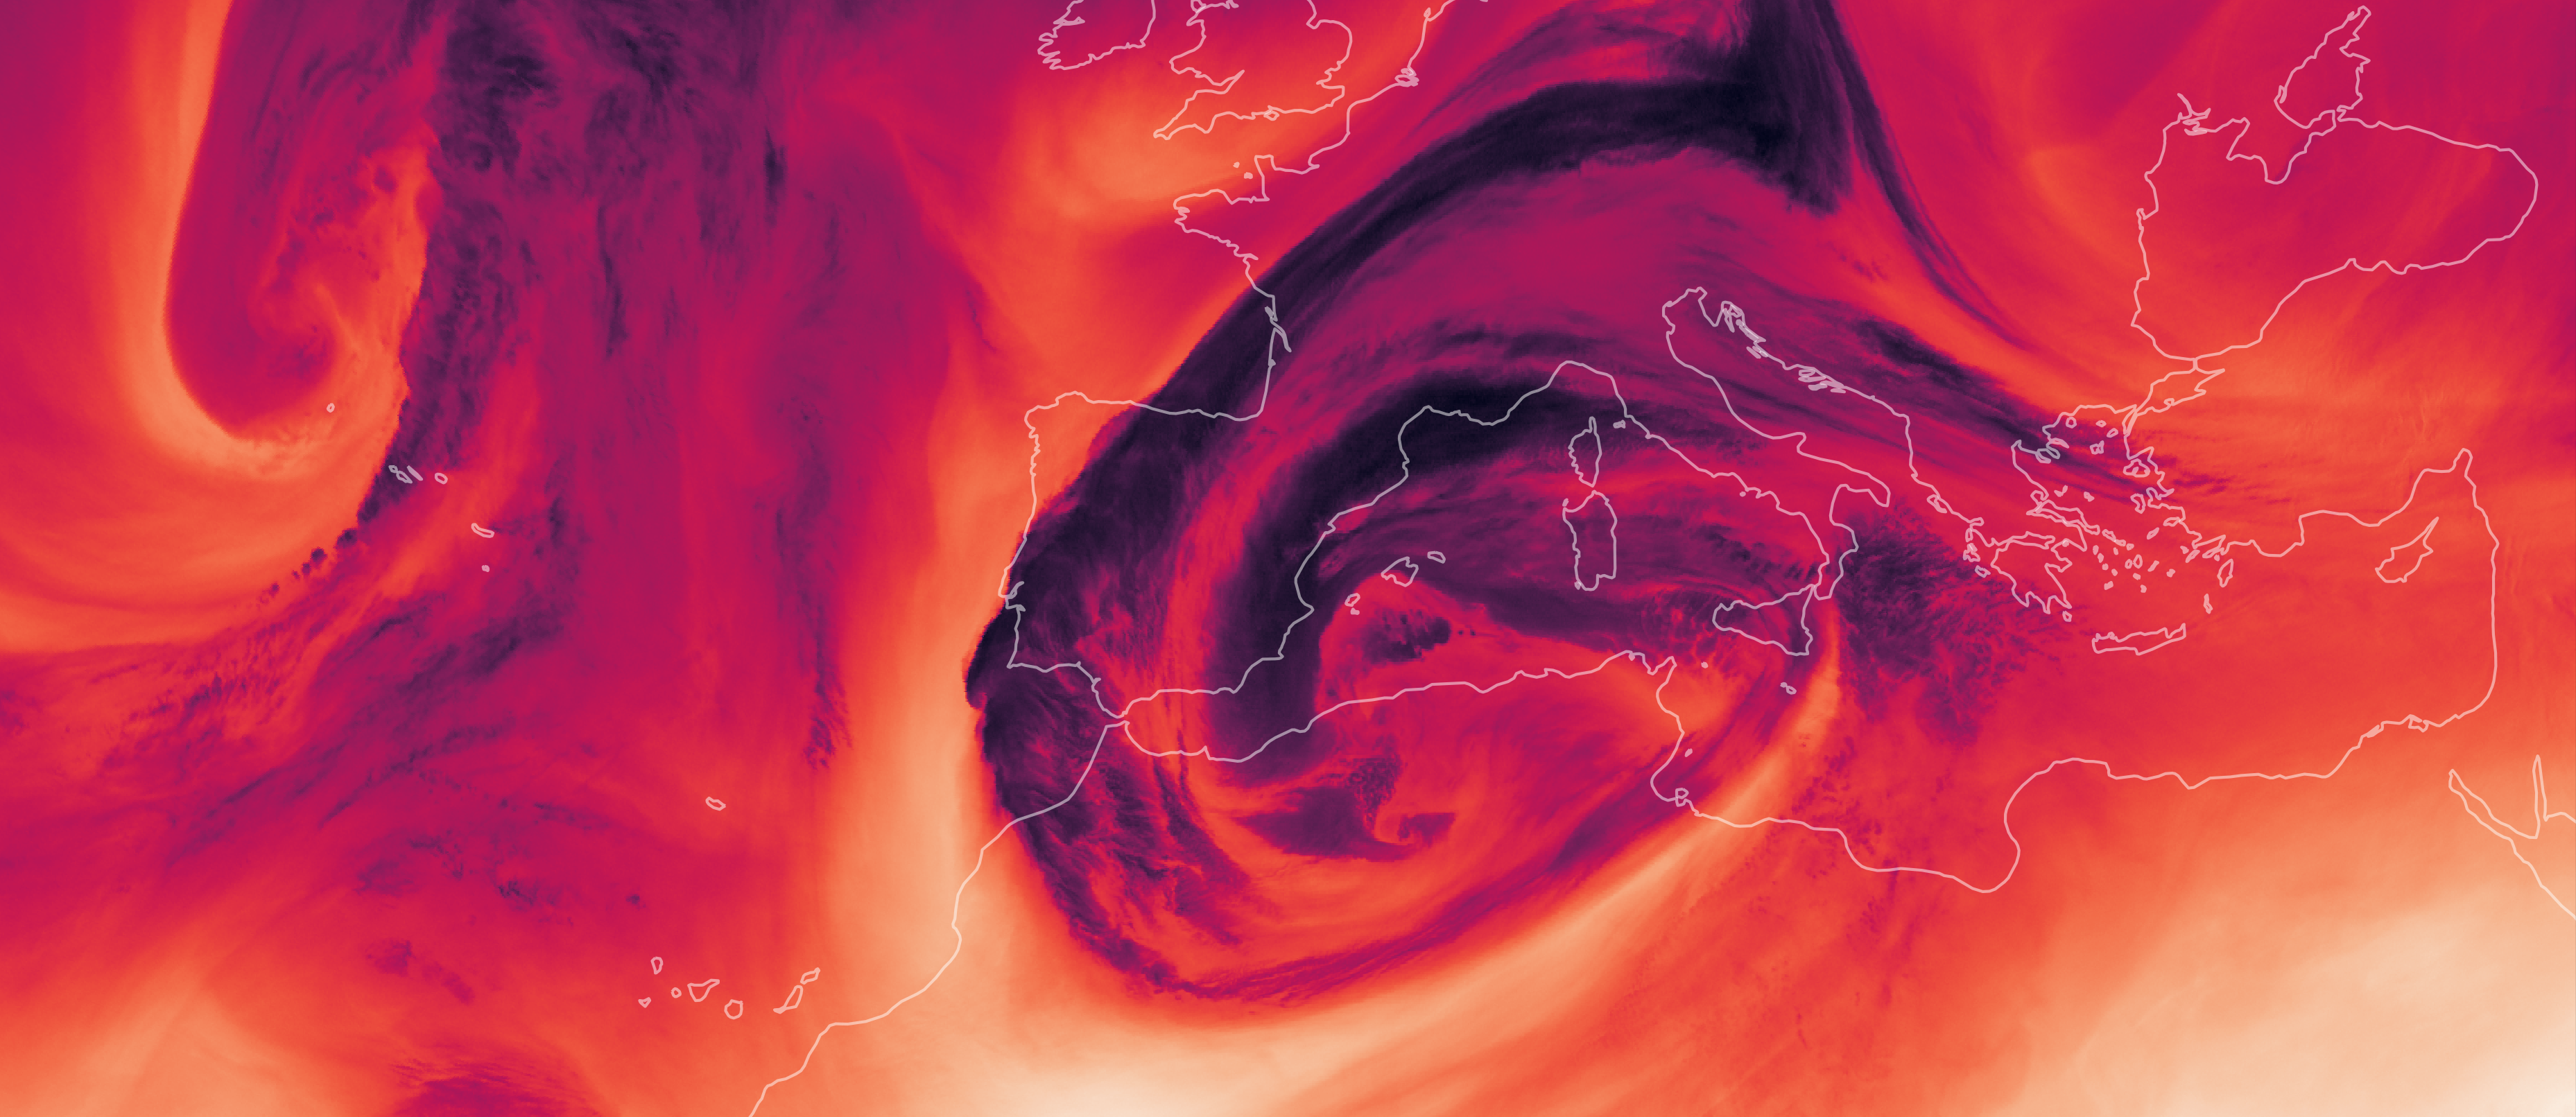
\includegraphics[width=\textwidth]{water_vapor}
\caption{Water vapor (white to red) and high clouds (purple to black) over the
Mediterranean as observed by the Spinning Enhanced Visible and Infrared
Imager at a wavelength of $\SI{6.2}{\micro \meter}$.}
\label{fig:introduction:water_vapor}
\end{figure}

This example illustrates that an understanding of the processes generating the
infrared radiation observed by a satellite, allows an observer to infer moisture
content as well as the presence of high clouds in the atmosphere. Formulated
more generally: If a component of the atmosphere interacts sufficiently strongly
with radiation, it generates an electromagnetic signal that can be measured
using a suitable sensor. By inverting the component's interaction with the
observed radiation, these measurements can be used to infer some of its
properties. This inversion process is called \textit{the retrieval} and is
required to relate satellite observations to the physical state of the
atmosphere.

The subject of this thesis are computational methods for retrieved properties of
clouds and precipitation from satellite observations. As will be explained in
more detail later on, these measurements are difficult, firstly, due to the high
variability in the appearance and composition of clouds and, secondly, due to
the complexity of their interaction with radiation. At the same time, the
important role that clouds and precipitation play in the weather and climate
system makes these measurements are highly relevant for science and society.

To set the scene for the discussion of satellite observations and retrieval
techniques in the subsequent chapters, this introduction aims to provide an
overview of the relevance of observing and measuring clouds and precipitation
from space. Beginning with the societal significance of water, the discussion
will move on to the scientific relevance of observing water as it moves through
the atmosphere.

\section{Water as resource}

Water is essential to life on Earth. It is the bloodstream of the biosphere
\citep{falkenmark04} and a fundamental resource to all forms of human
societies. The largest part of human freshwater consumption from lakes, rivers
or ground water, so called \textit{blue water} consumption, is used to irrigate
crops, while domestic and industrial use play minor roles. Blue water
consumption is distinguished from green water consumption, which refers to the
part of precipitation over land which is involved in the photosynthesis process.
Although rarely considered in consumption inventories, green water plays an
important role in providing water for rain-fed agriculture, which accounts $60$
to $\SI{70}{\percent}$ of the global food production, and in sustaining
terrestrial ecosystems \citep{falkenmark04}.

Humans thus depend on water for food production both through irrigation from
blue water flows as well as the provision of soil moisture by green water flows.
Achieving food security has been recognized by the United Nations (UN) as a
sustainable development goal (SDG, \citeauthor{sdg}, \citeyear{sdg}). The large
contribution of food production to overall water consumption poses a challenge
to the management of water resources. Diverting more blue or green water flows
to the production of food reduces the amount of water that is available to
sustain terrestrial and aquatic ecosystems. There is thus direct potential for
conflict between the SDGs to end hunger and the SDGs to sustain terrestrial and
aquatic ecosystems (13 and 14).

At the same time, water requirements for the production of energy are projected
to increase as fossil fuels are increasingly sourced from unconventional
deposits, such as shale oil and gas, whose extraction consumes substantial
amounts of water \citep{rosa18}. This is accompanied by a projected increase in
hydropower \citep{zarfl15} and the use of biofuels, both of which are reliant
on freshwater supplies. This emerging competition in water uses is recognized as
the \textit{food-energy-water} nexus \citep{dodorico18}.


% Also here satellite observations that allow
%the monitoring of water resource are an important tool for the effective
%management of droughts \citep{boyd13}.

%Water consumption is typically categorized into two classes: blue and
%green water consumption. Blue water consumption refers to 
%
%The consumption of water is typically categorized as blue water consumption,
%which refers to the extraction of surface water from rivers or ground water, and
%green water consumption, which refe to rain water consumed directly, for example
%to grow crops. Of the global blue water consumption, agricultural activity
%constitutes the largest part followed by industrial activity and domestic use
%\citep{falkenmark04}. Agriculture, however, also consumes large amounts of
%green water as $60$ to $\SI{70}{\percent}$ of the world's  food is produced on
%rainfed land.
%
%Water also plays an important role as source of energy. In the year 2020, energy
%produced from hydroelectric plants constituted one sixth of the global energy
%production \citep{eia21} and it can be expected that this portion will increase
%with the required decarbonization of the energy sector.


\section{The hydrological cycle}

Sustainable human water consumption depends on the replenishment of the sources
from which the water is obtained. Fresh water over land exists in the form of
glaciers, ice sheets, lakes and reservoirs, snow pack, wetlands and rivers as
well as a small part contained in the biomass. Water also exists within the land
surface in the form of soil moisture, permafrost and ground water. The largest
part of the water that is available on the surface of the Earth is stored in the
oceans. Compared to that, the part of water that is stored in the atmosphere is
very small. Most of that is in the form of water vapor while minor fractions are
contained in clouds as either liquid droplets or frozen ice
crystals \citep{abbott19}.

Despite containing only a tiny fraction of the global water reserves at any
given moment, the atmosphere is responsible for essentially all of the water
transport from oceans to land, where it replenishes the water storages from
which it is available for direct (blue) or indirect (green) consumption. The
system of fluxes between the different forms in which water exists on the
surface of the Earth is called the hydrological cycle.

The illustration in
\ref{fig:introduction:water_cycle} provides an overview of the principal fluxes
of the hydrological cycle. The largest flux is that from the ocean to the
atmosphere. A large part of the water vapor that evaporates of the ocean never
reaches the land but instead returns to the ocean in form of precipitation. Only
about $\SI{10}{\percent}$ of the evaporation over oceans is transported to land,
where it may precipitate to replenish land-based freshwater reserves. A part of
that precipitation evaporates again allowing it to take part in the formation of
precipitation further inland.

\begin{figure}
\centering
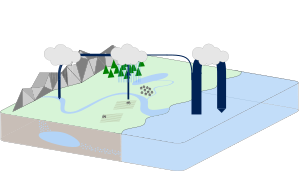
\includegraphics[width=0.8\textwidth]{water_cycle}
\caption{
Illustration of the global hydrological cycle. Water evaporates over the
Oceans and parts of it are transported to the land, where it fills up continental
water storages or re-evaporates.}
\label{fig:introduction:water_cycle}
\end{figure}

On the scale of river basins, the inflow of water through the atmosphere is the
only sustainable source of fresh water \citep{falkenmark04}. Given the competing
water requirements for the production of food, energy, the access to clean water
and the sustaining of ecosystems discussed above, it is clear that water
management is required to minimize conflicts and avoid human suffering. The
management of water resources in turn requires the monitoring and modeling of
the hydrological cycle. Since the fluxes of water in the atmosphere occur across
continental scales, the only currently available way of measuring them is with
the help of satellite observations.

\section{Weather and climate}

Water plays an important role in the weather system. When water evaporates, it
takes up energy from its environment. This energy, the latent heat, is released
when the air cools and the water vapor condensates. The release of latent heat
acts as fuel for the development of vigorous convective storms. The water that
is released by those storms in the form of precipitation can cause flooding and
land slides.

The ability to predict the weather has considerable value for society,
especially for high impact events involving extreme wind speeds or
precipitation. The availability of satellite observations has played an
important role in the steady improvement of weather forecast that occurred
during the last three decades
\citep{bauer15}. Weather forecasting  systems use satellite data to
determine a best estimate of the current state of the atmosphere, which is then
evolved into the future to predict the weather. While most advanced forecasting
systems ingest satellite observations directly and are thus not dependent on
satellite retrievals \citep{bauer10}, their use for improving model
initialization for short-range forecasts is still being investigated
\citep{dehaan14, benjamin21}. Besides that, retrievals of precipitation and
cloud properties are used by weather forecasters to gain situational awareness
and assess potential weather hazards.

%Despite the progress of the last decades, weather forecasts still struggle to
%produce accurate forecasts for specific meteorological contexts
%\citep{schafler18}. In many of those, the misrepresentation of the
%interaction of latent heat release through condensation and the large scale
%dynamics of the atmosphere were found \citep{rodwell13} to play a role.
%Improving the forecasts requires improving the representation of these processes
%in the model, which is where satellite-derived measurements of precipitation and
%clouds can help researchers better understand them.

Water is also an important actor in the climate system. It affects the Earth's
energy budget in multiple ways. Water vapor is the most potent greenhouse gas
and thus contributes strongly to the retention of radiative energy emitted from
the Earth's surface. In the form of clouds, water both cools the Earth system
through the reflection of solar radiation and warms it through the absorption of
upwelling longwave radiation. Although the global effect of clouds is a
pronounced cooling, the effect varies regionally and with the properties of the
clouds. Evaporation and transpiration are important for the transfer of heat
from the Earth's surface to the atmosphere. Since, on average, these two processes
have to be balanced by precipitation, the energy budget of the Earth is directly
linked to precipitation \citep{trenberth09}.

Instead of a passive tracer of atmospheric dynamics, the hydrological cycle must
thus be considered an active component of the both the weather and the climate
system. Both climate science and meteorology therefore rely on satellite observations
of the hydrological cycle to improve their understanding of the Earth system.


\section{A warmer planet}

As a consequence of anthropogenic emissions of carbon dioxide, the Earth's
 climate is heating up. As the Earth system adapts to the increased radiative
 forcing from greenhouse gases, its climate changes. These changes are not
 uniform but vary regionally and across spatial scales. Reliably regional
 predictions of climate change are required to help societies adapt to the
 changing climate. However, our current understanding as well us our ability to
 predict changes at regional scales remains severely limited.

Together with the climate, also the hydrological cycle is changing: Increased
evaporation leads to more frequent droughts at the same time as global
precipitation is expected to increase. Extreme precipitation events are
strengthening and becoming more frequent. The prediction of changes in the
hydrological cycle is complicated by their regional and scale dependence. At the
scales of individual precipitation systems, precipitation increases with the
capacity of warmer air to carry water vapor. Globally, however,
evapotranspiration and thus also precipitation are constrained by the Earth's
energy budget, which limits increases in global precipitation to a lower rate
than that of individual storms\citep{collins13}. These contrasting changes are
in turn modulated by changes in the general circulation, which ultimately
defines the global distribution of precipitation. Moreover, the detection and
prediction of these changes is difficult because on short time scales it likely
to be masked by the internal variability of precipitation.

As part of the hydrological cycle, clouds will change with the climate. Since
cloud reflect incoming solar radiation and the absorb outgoing long-wave
radiation, these changes act as a feed back on the Earth's energy budget and
will thus influence the response of the climate system to increased CO$_2$
concentrations. Whether an individual cloud exerts a net warming or cooling
effect on the climate system depends on its properties such as altitude and
composition as well as its location. The representation of clouds remains an
important challenge for climate models and uncertainties in cloud feedbacks
remain the primary source of uncertainty in predictions of the climate response
to increased CO$_2$ concentrations in the atmosphere \citep{zelinka20}.

Our understanding of climate change has progressed immensely during the last
decade but remains insufficient to make confident predictions at regional
scales. Such predictions are necessary for efficient climate change adaptation.
Satellite observations are therefore essential for improving and validating
climate models as well as the monitoring of changes in the climate system.


\section{Why satellites?}

Considering the importance of rain for a large range of human activities, it is
not surprising that humans have been measuring precipitation and trying to
improve their understanding of the weather system. The most direct and arguably
intuitive way to measure precipitation is through the use of \textit{rain
gauges}. A rain gauge consists of a cavity, which captures rain and from which
the accumulated precipitation can be measured. First records of gauge
measurements of rain date back to as long as 400 years
BC \citep{strangeways2000}. Today, gauge measurements are available from all
continents, however their density varies from country to country and is
oftentimes tied to the local population density.

The main disadvantage of rain gauges is the highly localized character of their
measurements, which limits their ability to accurately capture the spatial
structure of precipitation on short time scales. Moreover, because these
measurements are performed by a large number of public and private actors across
the globe, not all of them are easily accessible for scientists. Effectively,
only $\SI{1}{\percent}$ of the surface of the Earth is estimated to be within a
distance of $\SI{5}{\kilo \meter}$ from the nearest gauge
measurement \citep{kidd17}.

Over land, another important technique for measuring precipitation are
ground-based radars. These radars send out beams of radiation, which are
reflected by rain and snow. Precipitation within a radius several hundreds of
kilometers form the radar can be detected by measuring the amount of radiation
reflected back to the radar. Over land, ground-based radars play an important
role for real-time monitoring of precipitation. However, due to their high
installation and maintenance costs, their spatial availability is irregular and
typically tied to the local population density. In addition to that, the
availability and accuracy of radar measurements may be hampered by complex
terrain as well as the distance from the radar location, which limits the
usefulness of these observations for climatological applications.

The relevance of clouds and precipitation for the hydrological cycle has been
known since before the times of Aristotle \citep{frisinger72}. Nonetheless, the
systematic study of clouds has long remained a secondary focus of modern
meteorology and it took until the 1970s before the importance of interactions
between clouds, weather and climate put them at the forefront of atmospheric and
climate research \citep{stephens03}. Traditionally, cloud observations were
conducted as parts of routine meteorological observations performed on land and
ships \citep{hughes84}. However, these observations were mostly qualitative in
nature indicating only the presence of clouds, a cloud class and their rough
height.

The principal drawback of all of the measurement techniques discussed above is
their limited and irregular spatial coverage. This limits their value for the
monitoring of weather and climate. Satellites have the ability to provide
observations across global scales at high temporal resolutions. Because of this
they ideally complement ground based measurements and have become an essential
source of information for a wide range of scientific, economic and societal
activities.

